\newlength\colwidth
\newlength\topstripheight
\setlength{\colwidth}{.49\textwidth}
\setlength{\topstripheight}{.4\textheight}
% -----------------------------------------------------------------------
\fbox{%
\begin{minipage}[t][\topstripheight][t]{\colwidth}%
\begin{figure}[tb]
\def\PicWidth{0.24\textwidth}%
\centering%
\begin{subfigure}[b]{\PicWidth}
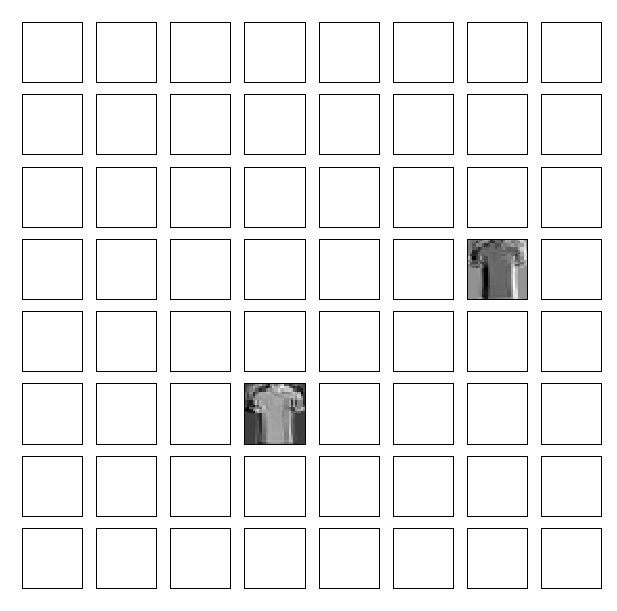
\includegraphics[width=\textwidth,trim=0.35cm 0.35cm 0.2cm 0.35cm,clip]{atelier/FMNIST/FM_e0.pdf}%
\caption{Iteration 0}
\end{subfigure}
\hfill%
%
\begin{subfigure}[b]{\PicWidth}
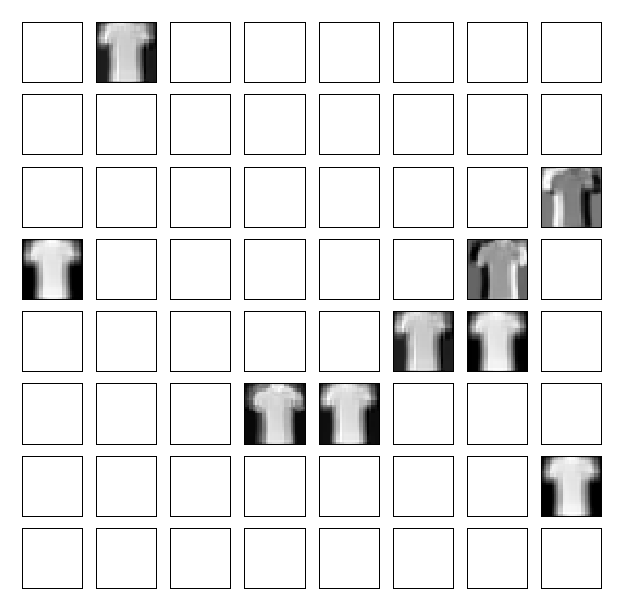
\includegraphics[width=\textwidth,trim=0.35cm 0.35cm 0.2cm 0.35cm,clip]{atelier/FMNIST/FM_e5.pdf}%
\caption{Iteration 5}
\end{subfigure}
\hfill%
%
\begin{subfigure}[b]{\PicWidth}
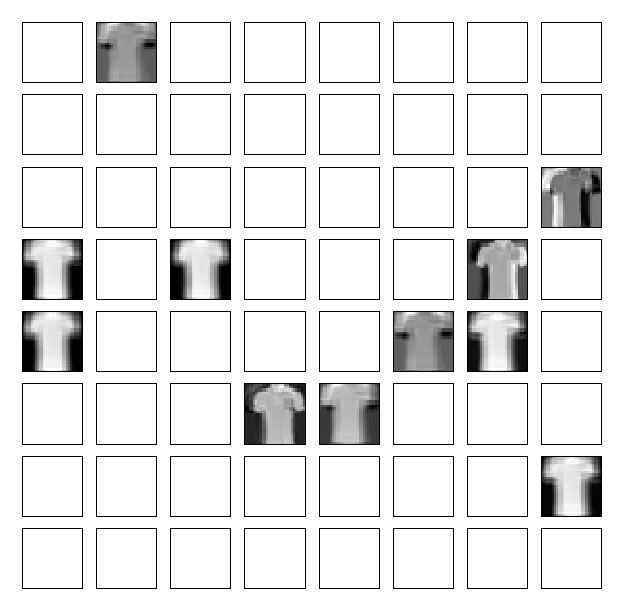
\includegraphics[width=\textwidth,trim=0.35cm 0.35cm 0.2cm 0.35cm,clip]{atelier/FMNIST/FM_e20.pdf}%
\caption{Iteration 20}
\end{subfigure}
\hfill%
%
\begin{subfigure}[b]{\PicWidth}
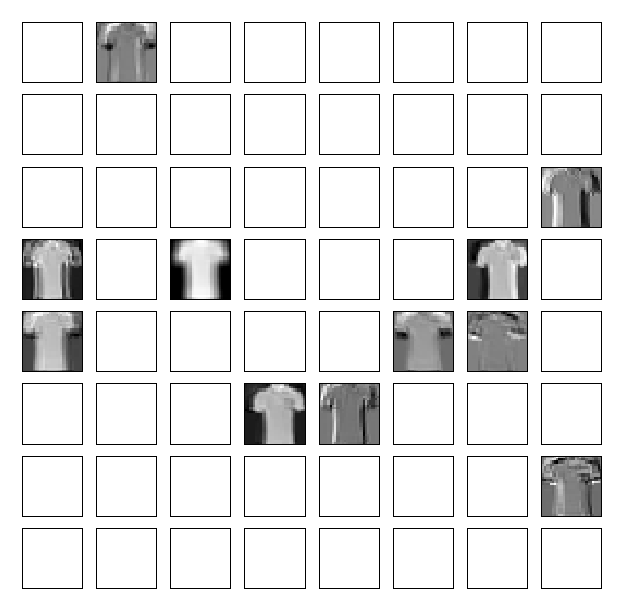
\includegraphics[width=\textwidth,trim=0.35cm 0.35cm 0.2cm 0.35cm,clip]{atelier/FMNIST/FM_e100.pdf}%
\caption{Iteration 100}
\end{subfigure}
\caption{Inverse scale space character of \LinBreg{} visualized through feature maps of a convolutional neural network. 
Descriptive kernels are gradually added in the training process.}
\label{fig:kernels}
\vspace{-10pt}
\end{figure}
%
%
%
%
\begin{block}{}%
$g \gets \nabla\empBatchLoss(\param;B)$ Backpropagation\\
$v \gets v - \tau g$ Gradient step\\
$\param \gets \prox{\delta\func}\left(\delta v\right)$ Regularization
\end{block}%
\end{minipage}%
}%
%
%
%
%
%
\hfill%
\fbox{%
\begin{minipage}[t][\topstripheight][b]{.005\textwidth}%
\begin{center}
\textcolor{BaseDarkColor}{%
\rule{.2mm}{\topstripheight}%
}
\end{center}
\end{minipage}%
}%
\hfill%
%
%
%
%
%
% --------------------------------------------------------------------------
% Analytical Results
\fbox{%
\begin{minipage}[t][\topstripheight][b]{\colwidth}%
\colorbox{BaseColor}{\makebox[\textwidth]{\textcolor{white}{Assumptions}\hfill}}\\

%
%
%
%
\colorbox{BaseColor}{\makebox[\textwidth]{\textcolor{white}{Loss Decay}\hfill}}\\
The iterates of ?? satisfy
\begin{block}{}
\begin{align*}
\E\left[\empLoss(\param^{(k+1)})\right] &+
%
\frac{1}{\tau^{(k)}}\E\left[ D^\mathrm{sym}_\func(\param^{(k+1)},\param^{(k)})\right]\\
%
&+
\frac{C}{2\delta\tau^{(k)}}\E\left[\norm{\param^{(k+1)}-\param^{(k)}}^2\right] \\
%
&\leq \E\left[\empLoss(\param^{(k)})\right] + \tau^{(k)}\delta\frac{\sigma^2}{2c},
\end{align*}
\end{block}
%
%
%
\colorbox{BaseColor}{\makebox[\textwidth]{\textcolor{white}{Convergence in Norm}\hfill}}\\
$J(\param^*)<\infty$ the stochastic linearized Bregman iterations ?? satisfy the following:
\begin{itemize}
\item Letting $d_k:=\E\left[D_{\func_\delta}^{v^{(k)}}(\param^*,\param^{(k)})\right]$ it holds
%
\begin{block}{}
\begin{align*}
&d_{k+1} - d_k\\
%
&+ \frac{\mu}{4}\tau^{(k)}\E\left[\norm{\param^*-\param^{(k+1)}}^2\right]\\
%
&\leq  \frac{\sigma}{2}\left((\tau^{(k)})^2 +\Exp{\norm{\param^{(k)} - \param^{(k+1)}}^2}\right).
\end{align*}
\end{block}
%
\item The iterates possess a subsequence converging in the $L^2$-sense of random variables: 
\begin{align*}
\lim_{j\to\infty}\E\left[\norm{\param^*-\param^{(k_j)}}^2\right] = 0.
\end{align*}
\end{itemize}
\end{minipage}%
}%

\fbox{%
\begin{minipage}{\textwidth}
Seperator
\end{minipage}%
}%


